\chapter{ランサムウェア対策}
\section{感染リスクの緩和}
現実世界の攻撃を戦術と使用技術の観点から分類したフレームワークであるMITRE ATT\&CK \cite{MITREATT12:online}によると,
ランサムウェアのデータ侵害は,攻撃の最終段階であるImpactステージの
Data Destruction,
Data Encrypted for Impact,
Data Manipulation
のいずれかに分類される.
つまり,ランサムウェアによるデータ侵害はInitial Access (初期アクセス) や Privilege Escalation (権限昇格) などのステージを完了した後に発生するといえる.
したがって,Impactより前のステージにおけるセキュリティ強化もランサムウェア対策の重要な要素である.
なお,本研究の提案手法はランサムウェアのImpactステージの活動に対する対策であるため,本節の内容はスコープ外であることに注意する.
\begin{figure}[t]
  \begin{center}
    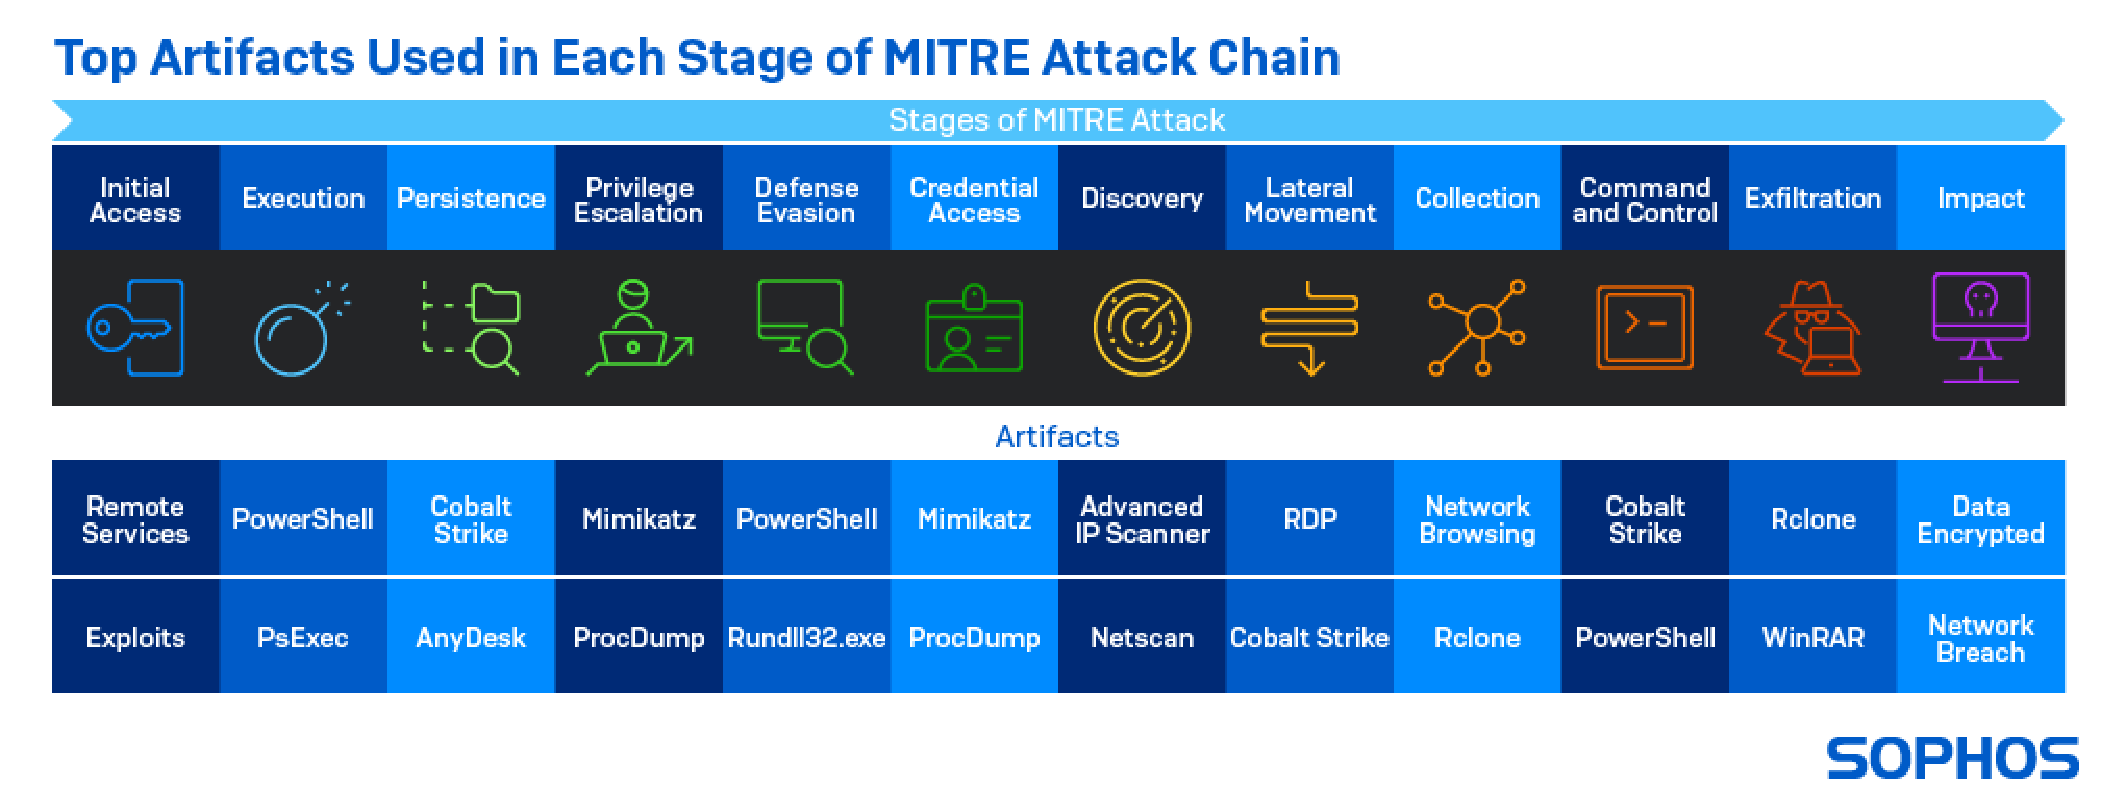
\includegraphics[width=\columnwidth]{doc/img/mitre-attack-chain.eps}
  \end{center}
  \caption{Overview of each stage in MITRE ATT\&CK framework.
    Some stages such as Reconnaissance are omitted for simplicity. \cite{mitre-explained}}
  \label{fig:mitre-attack-chain}
\end{figure}

本節では,すべてのランサムウェアが通過するステージであるInitial Accessステージに焦点を当て,感染リスクの緩和について述べる.
SpyCloud社 \cite{spycloud-ransomware} によると,ランサムウェアのInitial Accessに利用される手法として2023年に最も多く報告されたものは
フィッシング,サードパーティアプリケーションのIAM設定の不備(e.g. 過剰な権限付与),cookie窃取によるセッションハイジャックであった.
これらの手法に対する一般的な対策を\tabref{tab:initial-access}に示す.
\begin{table}[t]
  \centering
  \caption{Techniques for Initial Access and general countermeasures}
  \label{tab:initial-access}
  \begin{tabular}{|c|c|}
    \hline
    \textbf{Initial Accessの手法} & \textbf{対策} \\
    \hline
    フィッシング                     &
    \begin{tabular}{c}
      メールフィルタリングを強化する \\
      組織構成員の教育を行う
    \end{tabular}
    \\
    % Email filteringUser awareness training,         \\
    \hline
    IAM設定の不備                   &
    \begin{tabular}{c}
      多要素認証を導入する
      % Email filtering \\ User awareness training
    \end{tabular}
    \\
    \hline
    Cookie窃取によるセッションハイジャック     &
    \begin{tabular}{c}
      Secure属性やHTTPOnly属性を強制する \\
      多要素認証を導入する
    \end{tabular}
    \\
    \hline
  \end{tabular}
\end{table}

\section{ランサムウェア検知}
\label{sec:ransom-detect}
\subsection{検知に使用するデータ}
本稿において,
あるアプリケーションがランサムウェアであるかどうかを判断するための入力データを,
実行ファイルの解析から得られる静的データと,実行ファイルを実行した際にプロセスの振る舞いから得られる動的データに分類する.
\cite{berrueta2019survey}では検知のための入力データをlocal static (バイナリファイルの構造的特徴),
local dynamic (プログラム実行時の振る舞いから得られるデータ),
network based (実行中のプログラムが送信または受信するネットワークトラフィック)の3種類に分類しているが,
プログラム実行中に収集されるデータであることから,本稿ではネットワークトラフィックを動的データに含める.
\cite{Evolution-Ransomware}が調査した,ランサムウェア検知の先行研究において採用された技術および入力データの統計を\figref{fig:detection-overview}に示す.
\begin{figure}[t]
  \begin{center}
    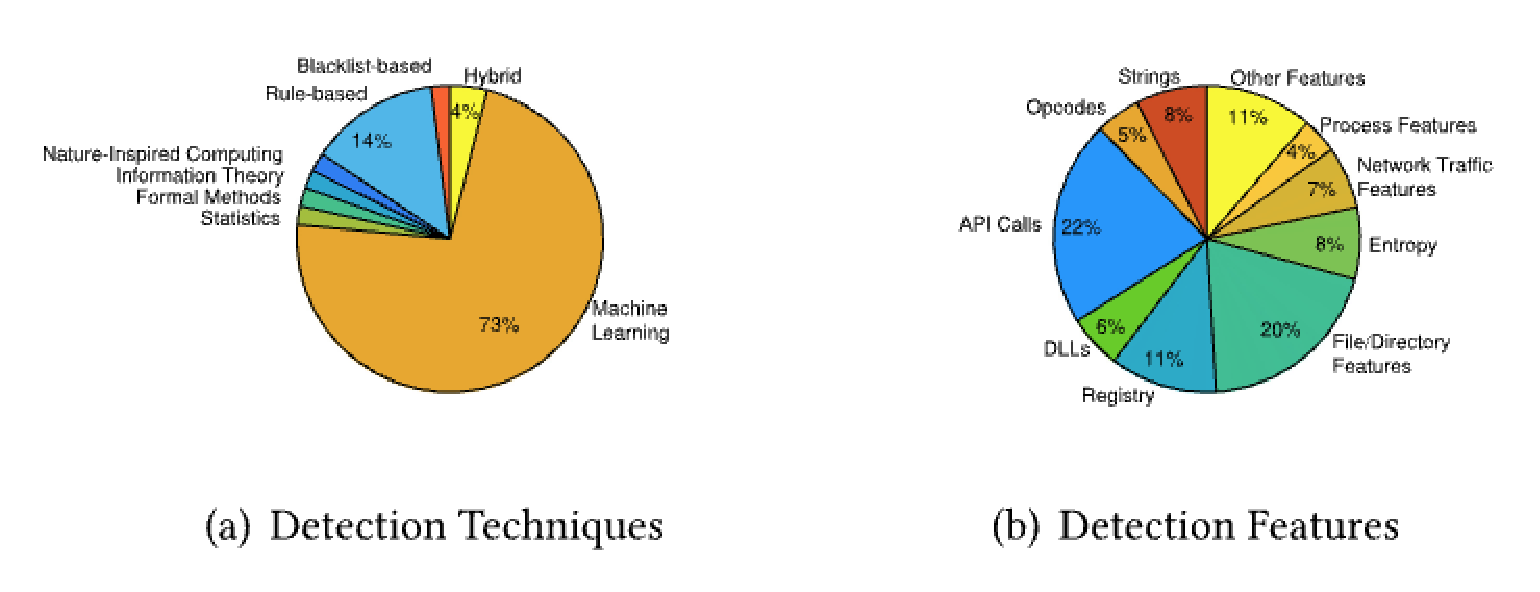
\includegraphics[width=\columnwidth]{doc/img/detection_overview.eps}
  \end{center}
  \caption{Distribution of detection techniques and detection features used in previous ransomware detection studies for PC/workstation. \cite{Evolution-Ransomware}}
  \label{fig:detection-overview}
\end{figure}


典型的な静的データはファイルのハッシュ値,文字列,ライブラリのAPI呼び出しなどである.
文字列としては"ransom"や"bitcoin"などのランサムノートに頻出する文字列,
過去にランサムウェアが使用していたドメイン文字列やIPアドレスなどが検知に利用されることが多い\cite{berrueta2019survey}.
しかし,静的データは一般に難読化や圧縮などの手法に弱く,さらに新種のランサムウェアに対して有効ではないことが多いという問題が指摘されている \cite{mitigation-modern}.
API呼び出しは,暗号化やファイルアクセスといった操作の有無をもとに,ランサムウェアと良性アプリケーションを区別するために
利用されることがある \cite{Evolution-Ransomware}.
API呼び出しの情報は,実行ファイルが使用するシステムライブラリから取得される.
これにはライブラリの情報が動的リンクまたは静的リンクとして実行ファイルに埋め込まれている場合を含む.
また,実行ファイルに含まれるオペコードも静的解析の対象となることがある \cite{baldwin2018leveraging}.

動的検知では実行中のプロセスの振る舞いを分析する.
典型的なランサムウェアは特定のディレクトリ以下のファイル一覧を取得して各ファイルを暗号化する挙動を繰り返し行うことから,
ファイルシステム上の操作,暗号化ライブラリやAPIの呼び出しが使用されることが多い \cite{Evolution-Ransomware}.
またランサムウェアがファイルに書き込むデータは暗号化されており情報学的エントロピーが高いため,
書き込まれるデータのエントロピーを利用する手法も複数存在する \cite{kharaz2016unveil,kharraz2017redemption}.
ただし書き込みデータのエントロピーはファイル圧縮などの正常アプリケーションにおいても高くなるので,エントロピーはその他の特徴量と組み合わせて使われる傾向がある \cite{berrueta2019survey}.
一部のランサムウェアは暗号化が完了したファイルの拡張子を変更する挙動を示すため,ファイル拡張子の変更も動的データとして利用されることがある\cite{medhat2018new}.
ネットワークトラフィックは,主にランサムウェアとC2サーバとの通信を検知するために使用可能である.
送信元や宛先のIPアドレス,ポート番号,プロトコル,ドメイン名が使用されることが多い\cite{Evolution-Ransomware}.

\subsection{代表的な検知手法}
% 検知手法の調査文献\cite{Evolution-Ransomware,berrueta2019survey,begovic2023cryptographic} を参考とした.
\subsubsection{機械学習による検知}
\figref{fig:detection-overview}が示すように,ランサムウェア検知のために機械学習が広く利用されている.
\cite{alraizza2023ransomware}は2017年から2022年までに提案された機械学習ベースの検知手法を調査しており,
本稿ではこの調査結果をもとに機械学習による検知手法を紹介する.

Baekら \cite{baek2018ssd} はSSD上のデータのランサムウェアによる上書きのパターンを検知するために,
SSD上にランサムウェア検知器を導入した.
筆者らはリクエストデータそのものではなく軽量なI/Oリクエストヘッダから検知を行うことで検知器のオーバーヘッドを改善している.
I/Oリクエストヘッダには論理ブロックアドレス,リクエストタイプ (read or write),データサイズのみが含まれており,
これらの情報から6種類の特徴量を作成して決定木に入力する.
SSD-Insiderはランサムウェアサンプルによる実験でほぼ0\%の誤検知率および見逃し率を達成し,
ランサムウェアに類似した高頻度の書き込みが行われるシナリオにおいても誤検知率は5\%未満に抑えられた.

機械学習ベースの検知手法では静的データと動的データを組み合わせることで検知精度の向上が得られることが多い\cite{alraizza2023ransomware}.
たとえばWangら \cite{wan2018feature}はユーザプロセスのパケットデータをフローに要約した動的データと
実行ファイル内の文字列やメタデータといった静的データを組み合わせて特徴量を作成し,
これをもとに決定木を用いてランサムウェア検知を行った.

\subsubsection{ルールベースの検知}
Medhatら \cite{yara-rule} はマルウェアの特徴を記述する文字列であるYARA \cite{yara-rule-doc} ルールを
自動生成してランサムウェア検知を行うシステムを提案した.
提案手法では実行ファイルの暗号ライブラリおよびファイル操作のAPI呼び出し,文字列を静的に解析することで,
解析対象のファイルに悪意スコアを割り当てる.
一方Redemption \cite{kharraz2017redemption} は,プロセスの振る舞いに基づく特徴量と
アクセスされたファイルコンテンツに基づく特徴量を利用してMSC (Malice Score Calculation, 悪意スコア計算) 関数を使用してランサムウェア検知を行った.
ユーザプロセスの悪意スコアはMSC関数によって計算され,閾値を超えた場合にランサムウェアと判定される.

\subsubsection{デコイファイルによる検知}
デコイファイルとは,正常なアプリケーションがアクセスしないように作成されたダミーファイルのことである.
あるプロセスがデコイファイルを上書きした場合,そのプロセスはランサムウェアである可能性が高いと考えられる.
RWGuard \cite{mehnaz2018rwguard} はプロセスおよびファイルの監視とデコイファイルを組み合わせた検知手法であり,
ランサムウェア検知におけるデコイファイルの効果を評価している.
具体的には,
事前定義されたファイルのみ暗号化するためデコイファイルにはアクセスしないランサムウェアや,デコイファイルの配置を認知している内部犯を想定して,
デコイファイルを使用する場合と使用しない場合の実験を行った.
その結果,デコイファイルはランサムウェアの検知を高速化するために有効であることが示された.

\subsection{検知レイテンシ}
動的検知あるいはハイブリッド検知において,ランサムウェアが実行されてから検知されるまでの時間を本稿では検知レイテンシと呼ぶ.
% 検知レイテンシは,小さいほどランサムウェアの被害を抑えることができるため,検知手法の評価指標として重要である.
検知レイテンシはランサムウェア攻撃を迅速に終了させられるかどうかという観点において重要な指標である.

RATAFIA \cite{alam2019ratafia} はオートエンコーダを用いた検知手法で,WannaCryを含む変種を最大5.3秒で検知した.
また,RWGuard \cite{mehnaz2018rwguard} はデコイファイル,プロセス監視,ファイル監視を組み合わせてレイテンシの削減を目指した手法であり,
評価実験ではランサムウェアのプロセスを9秒未満で特定した.
Brownorら \cite{brownor2024ransomware} は提案した検知手法の検知レイテンシをCPU使用率ごとに測定し,
使用率が90\%の設定でも評価に用いたランサムウェアサンプルを3秒未満で検知することができた.

検知レイテンシは検知手法の有効性を評価する上で重要な指標であるが,
検知レイテンシの評価を行っている研究が少ないことが指摘されている\cite{alam2019ratafia}.
例えばいくつかの研究では,提案手法の検知精度を最大化するために,30日間などの非常に長い期間での評価を行っているものがある \cite{mitigation-modern}.

\section{ランサムウェア被害からの復旧}
\label{sec:ransomware-recovery}
ランサムウェア被害からの復旧とは,ランサムウェアによって侵害されたデータを,\textbf{身代金を支払わずに}攻撃前の状態に戻すことを指す.
% したがって復旧手法は,データの復旧を実施するトリガとして,人間の明示的な入力または手法自体の自動的なランサムウェア検知を必要とする.
復旧手法を適用するには,手動での操作または自動的なランサムウェア検知によるトリガーが必要である.

\subsection{スナップショットによる復旧}
\label{subsec:snapshot}
スナップショットとは,特定の時点でのファイルシステムやデータの状態を記録する機能である.
ランサムウェア攻撃が発生する前に取得したスナップショットを用いることで,攻撃前の状態にデータを復元することができる.
そのため一定間隔でスナップショットを取得し,隔離されたストレージに保存しておくことはランサムウェア対策として広く採用されている \cite{wang2024ransom}.

ZFS \cite{openzfsz73:online} やBtrfs \cite{BTRFS—Th72:online}はファイルシステムとしてネイティブにスナップショット機能を提供している.
ZFSは差分スナップショット方式を採用しており,スナップショット取得後に更新されたファイルのみをCOW (Copy-On-Write) によってコピーする.
これによりスナップショット作成を高速に行い,ストレージ容量を節約している.
ZFSのスナップショットはファイルシステム単位で作成され,スナップショットを取得したファイルシステム上に保存される.
BtrFSもZFSと同様に差分スナップショット方式をサポートするが,スナップショットはサブボリューム単位で作成される.
サブボリュームはファイルシステム上でディレクトリとして扱えるデータ領域で,ユーザが作成・削除することができるため
ZFSよりも柔軟なスナップショット管理が可能である.

一部の商用OSはスナップショット機能を提供している.
WindowsのVSS (Volume Shadow Copy Service) はファイルシステムのスナップショットを取得する機能であり,
MacOSのTime Machineはファイルシステムに加えてアプリケーションや環境設定なども1時間ごとの差分バックアップにて保存する機能である.
なお,LockyなどのランサムウェアはVSSを削除することでスナップショットを無効化することがある \cite{Evolution-Ransomware}.

ハイパーバイザの機能を利用して仮想マシンまたは仮装ディスクのスナップショットを取得することもできる.
例えばXen Hypervisor \cite{xenHV}ではインターフェースなどのVMの設定情報を含むスナップショットを作成する機能を提供しており,
作成したスナップショットをもとにVMを新規作成したり,スナップショットをマージすることでデータを復元したりすることができる.
Azure \cite{azure-backup}などの主要なクラウドサービスプロバイダもユーザ使用する仮想マシンのOSおよび仮装ディスクのスナップショット取得機能を
提供している.
近年のクラウドサービスを対象としたランサムウェア攻撃の増加\cite{zscaler-ransomware}を受け,
ランサムウェア対策に特化したスナップショット機能を提供するクラウドストレージサービスも登場している \cite{huawei-solution}.



\subsection{暗号化鍵の取得による復旧}
\ref{subsec:encrypt-algo}節で述べたように,共通鍵暗号では暗号化と復号に同じ鍵を使用する.
そのため共通鍵暗号を利用するランサムウェアに対しては,暗号化に使用される鍵を取得することができればデータを復号することができる.
PayBreak \cite{kolodenker2017paybreak} はこの点に着目して開発された手法で,Windows OSが提供する暗号化ライブラリを
フックして暗号化鍵を取得する.
取得された鍵は事前にユーザが登録した公開鍵によって暗号化されたのち,追記のみが可能なデータストアに保存される.
\begin{figure}[t]
  \begin{center}
    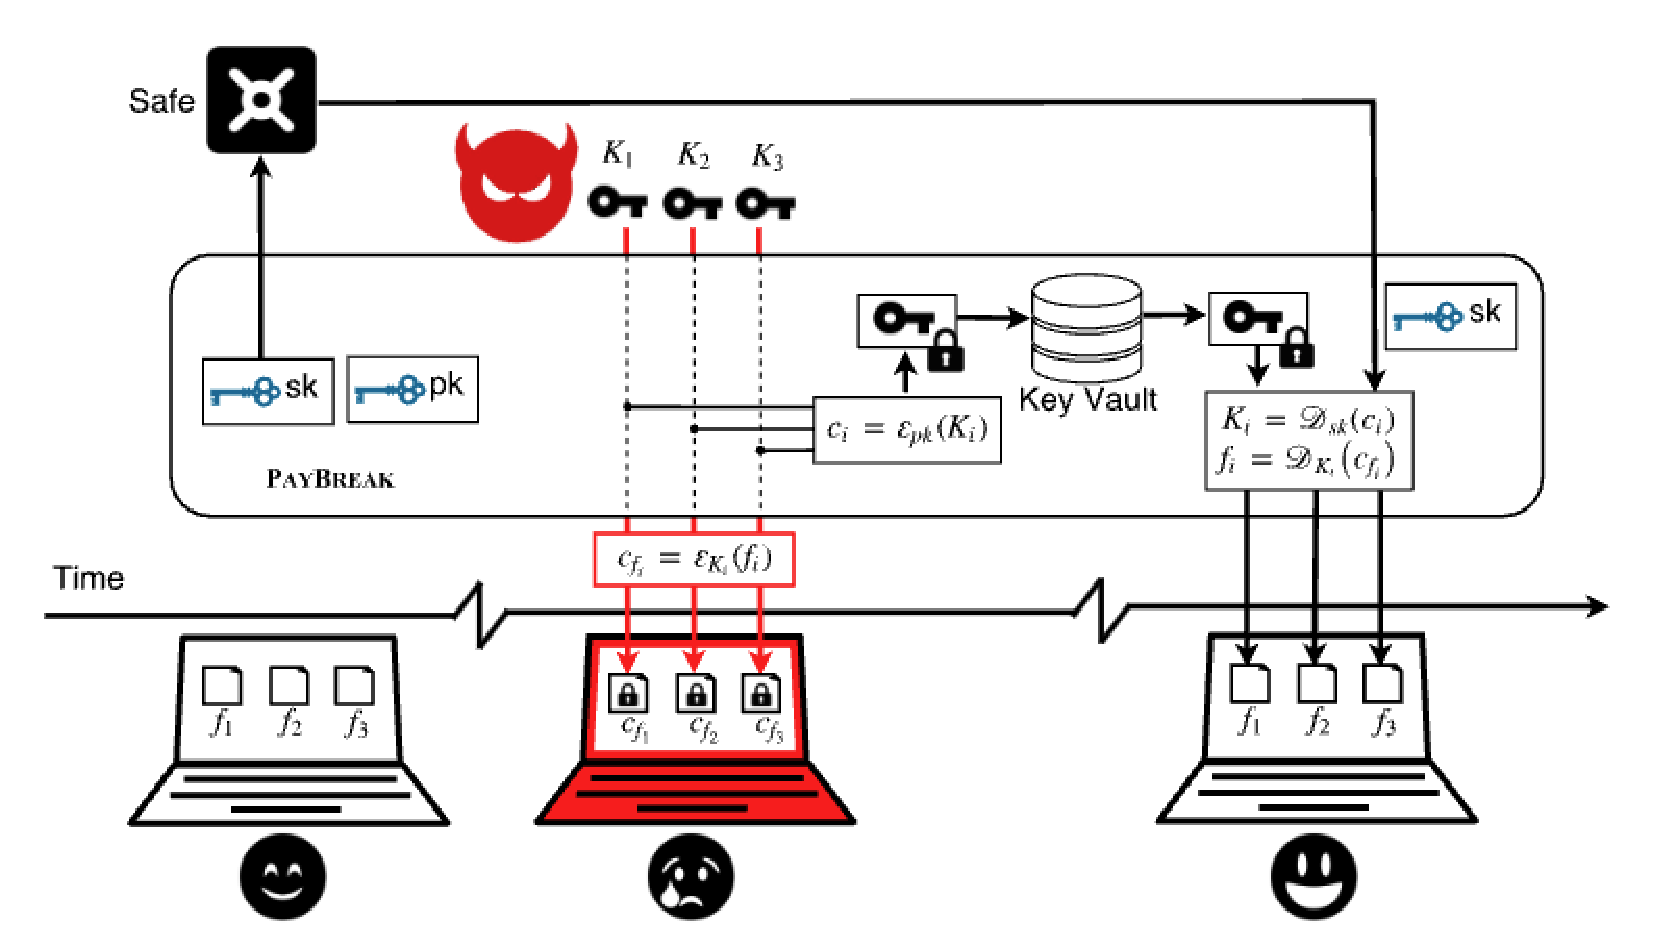
\includegraphics[width=\columnwidth]{doc/img/paybreak-overview.eps}
  \end{center}
  \caption{Overview of PayBreak. \cite{kolodenker2017paybreak}}
  \label{fig:paybreak-overview}
\end{figure}
PayBreakは暗号化ライブラリの動的リンクと静的リンクの両方に対応している.
さらに代替となる暗号化ライブラリが登場した場合でも,マルウェア解析によって一度暗号化関数を特定することができれば,
その関数をフック対象として容易に追加することができる.
しかしながら,PayBreakは非対称鍵暗号を利用するランサムウェアには対応していない.

\subsection{SSDの特性を利用した復旧}
\label{subsec:ssd-recovery}
SSDの特性を活用してランサムウェアにより侵害されたデータを復旧する手法が提案されている.
HDDとSSDはブロックデバイスとしての抽象化により論理的には同一のI/O操作を受け付けるが,
ハードウェアレベルではデータ上書き時の挙動が異なる.
HDDでは論理的な上書きに対して物理的な上書きが即時実行される (in-place書き込みされる) 一方で,
SSDにおける物理的な上書きは複数回の論理的な上書きに対してまとめて実行される
(上書きされる古いデータがout-of-place書き込みされ,GC: Garbage Collectionによって一定時間の後削除される).
これはSSD上で物理ページを消去するレイテンシが大きいためである.
つまり,SSDは上書きされたファイルや削除されたファイルのコピーを,GCまでの期間だけ保持することになる.

FlashGuard \cite{huang2017flashguard} は上記のSSDの特性を利用したデータ復旧システムであり,
SSDファームウェアとして実装された.
FlashGuardはランサムウェアによって上書きまたは削除された可能性のある物理ページに「GCによって回収しない」というフラグを立てることで,
SSD上にそのデータを保持してデータ復旧に使用できるようにする.
筆者らは1477個のランサムウェアサンプルを用いてFlashGuardの有効性を評価し,ランサムウェアによって暗号化されたファイルを効率的に復元可能であり
SSDに与える性能劣化も最小限であることを示した.

FlashGuardは保守的にデータの保持を行うため,実際には保持しておく必要がない古いデータまで保持してしまうという問題がある.
SSD-Insider \cite{baek2018ssd} はブロックI/Oリクエストのヘッダを参照してあるデータがランサムウェアによって侵害されたかどうかを判定することで
この問題を改善した.

SSDの特性を活用したこれらの手法は,ランサムウェア検知がデータ復旧のトリガとなるが,
検知において誤検知や見逃しが頻繁に発生する点が先行研究によって指摘されている \cite{han2020effectiveness}.
そのため本来必要のないリカバリが発生してデータが消失するリスクがある \cite{css2024-enomoto}.
さらに,ハードウェアに依存した復旧手法は大規模な展開が難しいという課題も指摘されている \cite{wang2024ransom}.
特殊なハードウェアまたはプロトタイプ的なハードウェアに依存していること,
ランサムウェアの進化に追随してファームウェアを頻繁に更新することが非現実的であるからだ.

\subsection{ファイルシステムの拡張による復旧}
いくつかの先行研究では,ファイルシステムを拡張することでランサムウェアによるデータ侵害からの復旧を実現している.
ShieldFS \cite{shieldFS} はOSのネイティブなファイルシステムにカーネルモジュールを適用し,
任意のプロセスのファイル書き込みまたは削除のI/Oリクエストに対してCOWを行うデータ保護システムである.
概要を\figref{fig:shieldFS}に示す.
ShiledFSはすべてのプロセスの低レベルのI/Oリクエスト,および不審なプロセスの暗号化処理を監視してプロセスごとの悪意スコアを計算するモジュールを持つ.
あるプロセスの悪意スコアが閾値を超えた場合,COWのコピー元となっているファイルを用いて,そのプロセスによって更新されたファイルを復旧する.
Redemption \cite{kharraz2017redemption} はShiledFSと類似した手法で,ファイルシステムへの書き込みおよび削除のI/Oリクエストをインターセプトし,
保護領域に作成されるコピーファイル (「リフレクションファイル」と呼ばれる) にリクエストをリダイレクトする.
リフレクションファイルは変更履歴が保持されており,ランサムウェアによるファイルの暗号化や削除を検知した場合,リフレクションファイルを用いてファイルを復元する.
\begin{figure}[t]
  \begin{center}
    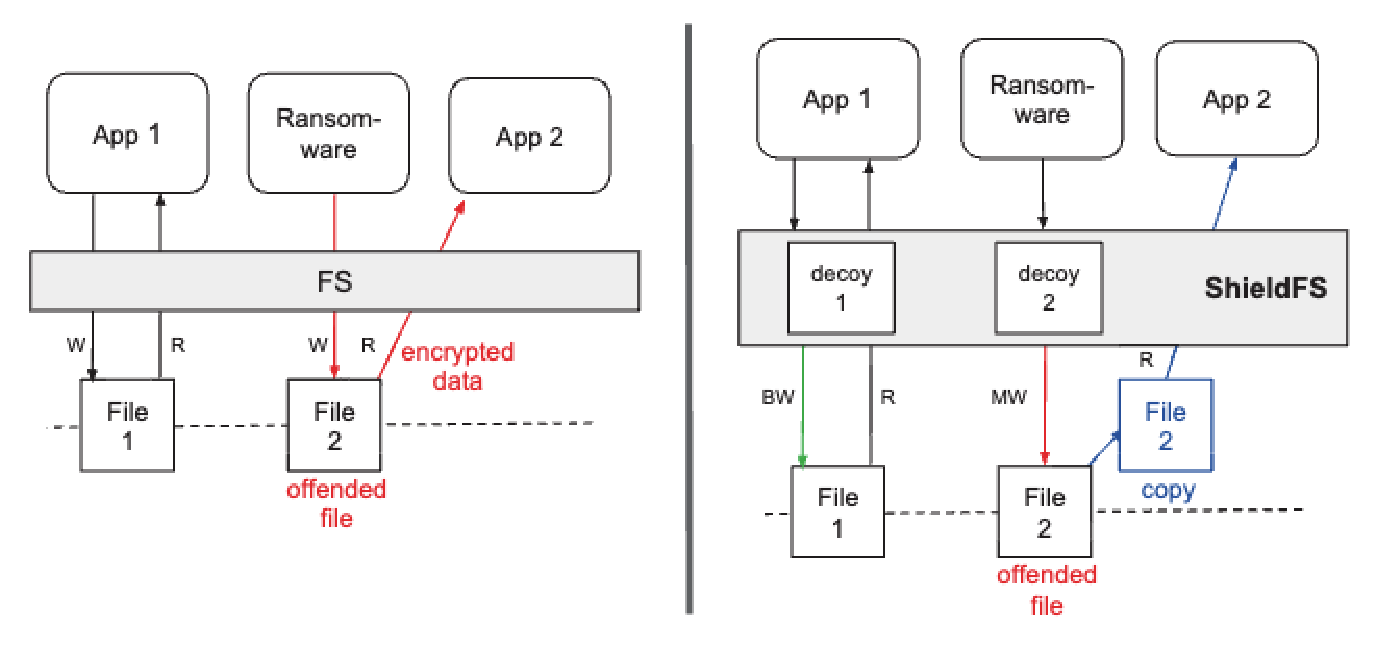
\includegraphics[width=\columnwidth]{doc/img/shieldFS.eps}
  \end{center}
  \caption{On the right ShieldFS shadowing a file offended by ransomware malicious write (MW), in comparison to standard filesystems (on the left). \cite{shieldFS}}
  \label{fig:shieldFS}
\end{figure}

MatosらはRockFS \cite{matos2018rockfs} を提案し,悪意ある第三者によるファイルデータの侵害からの復旧を行うシステムの設計と実装を行なった.
ランサムウェアなどがバックアップサービスのクライアントデバイス上に保存されているデータを侵害すると,データの更新がクラウドに同期されるため,
バックアップが利用不可能になってしまう.
RockFSは既存のクラウドバックアップサービスに存在するこの問題に注目し,
クライアントデバイス上のファイルシステム操作のログをクラウドストレージ上に保存するというアプローチを取っている.
ランサムウェア攻撃が発覚した場合に,ログ上の正常な操作のみをファイルの初期バージョンに適用することでデータを復元する.
攻撃者がクラウドストレージへのアクセス情報を窃取してログを改ざんすることを防ぐために,RockFSはログを完全性を保証するための手法を提案している.
さらにRockFSは操作ログを複数のクラウドストレージに分散して保存する仕組みを提供しており,ログの改ざんを試みる攻撃者は
複数のクラウドサービスに侵入する必要がある点が特徴的である.

\section{既存の復旧手法の課題}
\label{sec:recovery-challenges}
\subsection{スナップショットによる復旧の限界}
取得しておいたスナップショットを利用してデータをランサムウェア攻撃前の状態に復旧するためには
スナップショットを一定以上の頻度で取得しておく必要があるが,高頻度の取得には課題が伴う.
まず,金銭的なコストが大きくなる.
Wangら\cite{wang2024ransom}の試算によると,ALIBABA Cloudにおける仮想ディスクのスナップショット取得サービスを1時間ごとに利用する場合,
発生するコストは仮想ディスク使用料金の2.5倍に相当する.
このコストはスナップショット取得による追加のストレージ容量および処理時間によるものであるため,
クラウドサービスを利用せずオンプレミスでスナップショットを取得する場合でも同様のコストが発生する.

上述したコストを受容する場合でも,スナップショット方式による復旧ではデータ損失が発生する可能性が高いことが指摘されている\cite{wang2024ransom}.
第一に,最新のスナップショット取得時からランサムウェア攻撃発生までの間に更新されたデータは復旧されない.
第二に,\ref{subsec:snapshot}節で述べたように,スナップショットはファイルシステム,OS,ディスクなどの単位で取得される.
したがってスナップショットでは,ランサムウェアによって侵害されたデータと正常なアプリケーションによって更新されたデータが区別されずに
バックアップされる.
この性質により,データ更新が頻繁に発生する環境においてスナップショットによるデータのコピーがデータ更新に追いつかず,
データ損失が発生するおそれがある.

\subsection{復旧のトリガとなる検知の課題}
% ランサムウェア攻撃によるデータ侵害の復旧には,復旧のトリガとなるランサムウェア検知が必要である.
ランサムウェア検知手法は一般に誤検知と見逃しのトレードオフに悩まされる \cite{Evolution-Ransomware,berrueta2019survey, mitigation-modern}.
攻撃を見逃すと侵害されたデータの復旧が不可能になるため見逃し率は可能な限り小さくする必要があるが,
その場合トレードオフにより誤検知率が高くなり,正常なアプリケーションがランサムウェアとして判定され,システムの可用性が低下するおそれがある.
また\ref{subsec:ssd-recovery}で述べたSSDベースの手法 \cite{huang2017flashguard,baek2018ssd} にて誤検知が発生した場合,
誤ったデータ復旧によってデータが消失する危険性が指摘されている \cite{css2024-enomoto}.

実行時の振る舞いからランサムウェアを検知する手法では,必然的に一定時間のランサムウェアの活動を許容する.
被害を最小限に抑えるためには検知までの時間,検知レイテンシを短縮することが重要であるが,
短時間での検知では誤検知率および見逃し率が高くなると考えられる \cite{mitigation-modern}.
あるプロセスがランサムウェアであるかどうかを判定するための情報が不足するほか,
ランサムウェアが実行後すぐにデータ暗号化などの特徴的な挙動を行うとは限らないからだ.
